 %%%%%%%%%%     PREÁMBULO      %%%%%%%%%%%%%%%

%%%%%%%%%   Non modificar este preámbulo, salvo que se sepa ben o que se está a facer   %%%%%%%%%

%%%%%%  Traballando nun Mac, se usas TeXShop, en  Preferencias -> Código -> codificación de  caracteres (UTF-8)  %%%%

\documentclass[11pt,a4paper]{book}

% Formato do documento
\usepackage[papersize={210mm,297mm},lmargin=2.5cm,rmargin=2.5cm,top=3.5cm,bottom=3.5cm]{geometry}   % Marxes
\renewcommand{\baselinestretch}{1.25}                                                               % Fixamos o interliñado
\setlength{\parskip}{8pt}                                                                           % Separación entre parágrafos


\usepackage{amsmath,amsfonts,amssymb,amsthm}
\usepackage{latexsym,pdfsync,xcolor,graphicx}
\usepackage[nottoc]{tocbibind}
\usepackage[T1]{fontenc}
\usepackage[utf8]{inputenc}
\usepackage[spanish]{babel}			
\usepackage{tikz}
\usepackage{appendix}
\usepackage{hyperref}

\usepackage{pgfplots}

\usepackage{algpseudocode}
\usepackage{enumitem}
\newlist{steps}{enumerate}{1}
\setlist[steps, 1]{label = Paso \arabic*., leftmargin=2.6cm, topsep=0pt}

\usepackage{xfrac}
%\usepackage{listings}
\usepackage{matlab-prettifier}

\usepackage{calligra} % for dedication


% Cabeceira
\usepackage{fancyhdr}
\pagestyle{fancy}
\fancyhf{}
\renewcommand{\chaptermark}[1]{\markboth{\textbf{\thechapter. #1}}{}} % Formato para o capítulo: N. Nome
\renewcommand{\sectionmark}[1]{\markright{\textbf{\thesection. #1}}}  % Formato para a sección: N.M. Nome

\fancyhead[LO]{\rightmark}           % Nas páxinas impares, parte esquerda do encabezado, aparecerá o nome do capítulo
\fancyhead[RE]{\leftmark}            % Nas páxinas pares, parte dereita do encabezado, aparecerá o nombre da sección
\fancyhead[RO,LE]{\textbf{\thepage}} % Números de páxina nas esquinas dos encabezados




%%%   \pagestyle{plain}   Cando os títulos dos capítulos son moi longos, a opción por defecto das cabeceiras pode ser inapropiada;
%%%  nestes e noutros casos semellantes, pódese usar a opción "plain", que suprime as cabeceiras, deixando soamente a numeración das páxinas.


%%%%%%%      NON ESCRIBIR AQUÍ  (COMANDO PORTADA) %%%%%%%%%%%

\newcommand{\portada}[3]{
\thispagestyle{empty}

\definecolor{azulUSC}{RGB}{13,38,120}


\includegraphics[width=13cm]{logomath.pdf}

\vspace*{2cm}

\centerline{{\Large\bf  Traballo Fin de Grao}}

\vspace{2.6cm}

{\center{\Huge\bfseries\color{azulUSC} #1}\par}		

\vspace{1cm}

{\Large

\centerline{#2}		

\vspace{6.4cm}

\centerline{\sf #3}        

\vspace{1.25cm}

\centerline{\sf UNIVERSIDADE DE SANTIAGO DE COMPOSTELA}
}

\enlargethispage{1cm}
\clearpage
}

%%%%%%%      NON ESCRIBIR AQUÍ  (COMANDO PRIMEIRA PÁXINA) %%%%%%%%%%%

\newcommand{\primeira}[3]{
\thispagestyle{empty}
\enlargethispage{1cm}
\begin{center}\Large

{\sf GRAO DE MATEM\'ATICAS}

\bigskip
{\bfseries Traballo Fin de Grao}
\vspace{4cm}

{\bfseries\Huge #1} 		
\vspace{1.2cm}

{#2}		\par		     
\end{center}

\vspace{6.5cm}

\begin{center}
\Large
{#3}	\par			    

\vspace{1cm}
{\sf UNIVERSIDADE DE SANTIAGO DE COMPOSTELA}
\end{center}
\clearpage
}

%%%%%%%    Teoremas   %%%%%%%%%

\newtheorem{theorem}{Teorema}[chapter]
\newtheorem{proposition}[theorem]{Proposición}
\newtheorem{lemma}[theorem]{Lema}
\newtheorem{corollary}[theorem]{Corolario}
\newtheorem{algorithm}[theorem]{Algoritmo}
\newtheorem{axiom}[theorem]{Axioma}
\newtheorem{case}[theorem]{Caso}
\newtheorem{conclusion}[theorem]{Conclusión}
\newtheorem{condition}[theorem]{Condición}
\newtheorem{conjetura}[theorem]{Conjetura}				
\newtheorem{criterion}[theorem]{Criterio}
\newtheorem{ejercicio}[theorem]{Ejercicio}	
			
\theoremstyle{definition}
\newtheorem{definition}[theorem]{Definición}
\newtheorem{ejemplo}[theorem]{Ejemplo}				
\newtheorem{agradecimientos}[theorem]{Agradecimientos}	

\theoremstyle{remark}
\newtheorem{remark}[theorem]{Observación}
\newtheorem{notation}[theorem]{Notación}
\newtheorem{problem}[theorem]{Problema}
\newtheorem{solution}[theorem]{Solución}

\addto\captionsspanish{
	\renewcommand{\contentsname}{\'Indice} 
	\renewcommand\appendixname{Anexo}
	\renewcommand\appendixpagename{Anexos}
}


%%%%%%%%%%%%%%%%%%   Fin do Preámbulo   %%%%%%%%%%%%%%%%

\newcommand{\norm}[1]{\left\lVert#1\right\rVert}
\newcommand{\sucesionxk}{\left\{x_k\right\}}
\newcommand{\sucesion}[1]{\left\{#1\right\}}

\def\code#1{\texttt{#1}}

\begin{document}
\frontmatter

%%%%%%%%%%%      PORTADA      %%%%%%%%%%%%

\portada
{Resolución numérica del problema no lineal de mínimos cuadrados.\vspace{5pt}
Aplicaciones a la estimación de parámetros de modelos matemáticos.}		%  escribir aquí o  Título
{Dídac Blanco Morros}		%  escribir aquí o/a  Autor/a
{Curso Acad\'emico}		  	%  escribir aquí a Data de presentación, na forma:  mes, ano

%%%%%%%%     PRIMEIRA PÁXINA    %%%%%%%%%%%%%%%%%%

\mbox{}
\thispagestyle{empty}
\clearpage

\setcounter{page}{1}

\primeira
{Resolución numérica del problema no lineal de mínimos cuadrados. 
Aplicaciones a la estimación de parámetros de modelos matemáticos.}		%  escribir aquí o  Título
{Dídac Blanco Morros}		%  escribir aquí o/a  Autor/a
{Febrero, 2022}		  	%  escribir aquí a Data de presentación, na forma:  mes, ano

\thispagestyle{empty}

%%%%%%%%%%%      PROPOSTA DE TRABALLO      %%%%%%%%%%%%%%%%

\vspace*{.5 cm}

\chapter*{Trabajo propuesto}

\vspace{1 cm}

\begingroup
\renewcommand*{\arraystretch}{2.2}
\begin{tabular}{|l|}
	\hline
	
	{\bf \'Area de Co\~necemento:  \/ Matemática Aplicada}\\ \hline
	\begin{minipage}{11.5cm}
		{\vspace*{.2cm}
			\bf T\'{\i}tulo:   \/ \bf Resolución numérica do problema non linear de mínimos cadrados. Aplicacións á estimación de parámetros de modelos matemáticos.
			\vspace{.2cm}}
	\end{minipage}\\ \hline
	\bf Breve descrici\'on do contido\\ \hline
	\begin{minipage}{11.5cm}
		{\vspace*{.2cm}
O problema non linear de mínimos cadrados xurde en moitas aplicacións da ciencia e da enxeñería:
no axuste dun conxunto de datos a un modelo matemático, na estimación de parámetros,
na aproximación de funcións, etc. O obxectivo do traballo fin de grao é o estudo de métodos
numéricos para abordar o problema de minimización resultante. centrándose especialmente no
algoritmo de Levenberg-Marquardt. O estudante estudará o método, no marco dos métodos de
optimización con rexión de confianza e familiarizarase co seu uso mediante o comando
Isqnonlin de Matlab. As metodoloxías estudadas aplicaranse a exemplos académicos e á
estimación de parámetros de distintos modelos matemáticos a partir de datos experimentais.
		\vspace{.2cm}}
	\end{minipage}\\ \hline
	{\bf Recomendaci\'ons}\\ \hline
	\begin{minipage}{11.5cm}
		{\vspace*{.2cm}


		\vspace{.2cm}}
	\end{minipage}\\ \hline
	{\bf Outras observaci\'ons}\\ \hline
	\begin{minipage}{11.5cm}
		{\vspace*{.2cm}


			\vspace{.2cm}}
	\end{minipage}\\ \hline
\end{tabular}
\endgroup

\clearpage

\thispagestyle{empty}

\tableofcontents

\clearpage

\thispagestyle{empty}

\mbox{}

\clearpage

%%%%%%%%%     RESUMO---RESUMEN---ABSTRACT     %%%%%%%%%%%%%

\phantomsection
\addcontentsline{toc}{chapter}{Resumen}		
\chapter*{}

\section*{Resumen}

% escribir aquí resumo en español




\vspace{1.5cm}

\section*{Abstract}



% escribir aquí resumo en inglés



\clearpage

\thispagestyle{empty}

%%%%%%%%%    INTRODUCIÓN     %%%%%%%%%%%%%%%%%%
%%%%%%%%%    De non incluír unha INTRODUCIÓN, suprímese    %%%%%%%%%%

\phantomsection
\chapter*{Introducci\'on}\addcontentsline{toc}{chapter}{Introducci\'on}

\markboth{INTRODUCCI\'ON}{INTRODUCCI\'ON}

%%%%%%%%%%%     fin da INTRODUCIÓN     %%%%%%%%%%%%%

\mainmatter

%%%%%%%%%%%%%%%%%%%%%%%%%%%%%%%%%%%%%%%%%%%%%%%%%%%%%				S
%%%%%%%%%%%%%%%%%%%%%%%%%%%%%%%%%%%%%%%%%%%%%%%%%%%%%				 T
%%%%%%%%%%%%%%%%%%%%%%%%%%%%%%%%%%%%%%%%%%%%%%%%%%%%%				  A
%%%%%%%%%%%%%%%%%%%%%%%%%%%%%%%%%%%%%%%%%%%%%%%%%%%%%				   R
%%%%%%%%     Póñense os Capítulos    %%%%%%%%%%%%%%%				    T



\chapter{Fundamentos de la optimización sin restricciones}
% El problema de los mínimos cuadrados es un caso particular de optimización sin restricciones, y es por ello que comenzaremos introduciendo sus fundamentos. Ya que el problema de mínimos cuadrados es usado en multitud de campos para estimar parámetros, este es de los más utilizados dentro de los problemas de optimización sin restricciones.

Un problema de optimización sin restricciones tiene la forma 
\begin{equation}
	\min_{x}f\left(x\right),
	\label{eq:minf}
\end{equation}
donde $x\in\mathbb{R}^{n}$ y $f : \mathbb{R}^{n} \rightarrow \mathbb{R}$ es continuamente
diferenciable, a f se le llama \textbf{función objetivo}. 
Notar que podemos usar esta formulación para referirnos tanto a los problemas de minimización
como de maximización, basta sustituir $f$ por $-f$. 

La dificultad de un problema como este viene por no conocer el comportamiento
global de $f$. Normalmente solo disponemos de la evaluación de f en algunos puntos y,
a lo mejor, de algunas de sus derivadas. El trabajo de los algoritmos de
optimización es identificar la solución sin usar demasiado tiempo ni almacenamiento computacional.
Veamos una serie de definiciones y resultados necesarios.
 
\begin{definition}
	A una aplicación $\Vert \cdot \Vert$ se le llama \textit{norma} si y sólo si cumple:
	\vspace{-0.4cm}
	\begin{enumerate}
		\item $\norm{x} \geq 0, \: \forall \mathbb{R}^n$ y $\norm{x}=0$ si y solo si $x=0$.
		\item $\norm{\alpha x} = \vert \alpha \vert \norm{x},\: \forall \alpha \in \mathbb{R},\: x\in \mathbb{R}^n.$
		\item $\norm{x+y} \leq \norm{x} + \norm{y}, \forall x,y \in \mathbb{R}^n$.
	\end{enumerate}
\end{definition}

Un ejemplo muy común es la
\textit{norma} $l_2$, también llamada \textit{norma euclídea}, a la cual nos referiremos cuando no se especifique lo contrario, se define
\begin{equation}
		\norm{x}_2 = \left( \sum_{i=1}^n \vert x_i \vert^2 \right)^{\frac{1}{2}}.
\end{equation}

\begin{definition}
	Un punto $x^*$ se dice \textit{mínimo local} si existe $\delta > 0$ tal que $f(x^*) \leq f(x)$ para todo $x \in \mathbb{R}^n$ que satisface $\Vert x - x^* \Vert < \delta$.
	Un punto $x^*$ se dice \textit{mínimo local estricto} si existe $\delta > 0$ tal que $f(x^*) < f(x)$ para todo $x \in \mathbb{R}^n$ que satisface $\Vert x - x^* \Vert < \delta$ con $x \neq x^*$.
\end{definition}

\begin{definition}
	Un punto $x^*$ se dice \textit{mínimo global} si $f(x^*) \leq f(x)$ para todo $x \in \mathbb{R}^n$.
	Un punto $x^*$ se dice \textit{mínimo global estricto} si $f(x^*) < f(x)$ para todo $x \in \mathbb{R}^n$ con $x \neq x^*$.
\end{definition}


%% REPASO DE ALGORITMOS

%% \section{Generalidades de los algoritmos}

%% histórico??
% referencia 	NOCEDAL 2.2

\begin{definition}
	Sea $f: \mathbb{R}^n \rightarrow \mathbb{R}$ diferenciable en
$x \in \mathbb{R}^n$ tal que $\langle \nabla f(x), d \rangle < 0$, entonces a $d$ se le llama \textit{dirección descendente} de $f$ en $x$.
\end{definition}

\begin{theorem}[Teorema de Taylor] %% COMPATIBILIZAR CON RESULTADO ANTERIOR
	
	Sea $f: \mathbb{R}^n \rightarrow \mathbb{R}$ continuamente diferenciable y sea $p \in \mathbb{R}^n$, tenemos que 
	\begin{equation}
		f(x+p) = f(x) + \nabla f(x+tp)^Tp, \quad t\in (0,1).
	\end{equation}
	Si además, $f$ es dos veces continuamente diferenciable
	\begin{equation}
		\nabla f(x+p) = \nabla f(x)
		+ \int_0^1 \nabla^2 f(x+tp)p\:dt,
	\end{equation}
	y
	\begin{equation}
		f(x+p) = f(x) + \nabla f(x)^Tp
		+ \frac{1}{2}p^T \nabla^2 f(x+tp)p, \; t\in (0,1).
		\label{eq:thty}
	\end{equation}
\end{theorem}


\begin{proposition}
Partiendo de la reformulación de (\ref{eq:thty}) y teniendo en cuenta que el último término
es el error de aproximación $o(t)$
\begin{equation}
	f(x_k + td) = f(x_k) + t \nabla f(x_k)^Td + o(t),
\end{equation}
se cumple que
\begin{equation}
	\exists \delta > 0 \text{ tal que } f(x_k + td) < f(x_k)
	\quad \forall t \in (0, \delta)
\end{equation}
si y solo si $d$ es una dirección descendiente de $f$ en $x_k$.

\end{proposition}

Tratemos ahora las condiciones de optimalidad.

\begin{theorem}[Condición Necesaria de Primer Orden]
	Sea $f:D\subset \mathbb{R}^n \rightarrow \mathbb{R}$ continuamente diferenciable en un
	conjunto abierto $D$. Si $x^*$ es un mínimo local de (\ref{eq:minf}), entonces
	$\nabla f(x^*) = 0$.
\end{theorem}

\begin{theorem}
	(Condición Necesaria de Segundo Orden)
	Sea $f:D\subset \mathbb{R}^n \rightarrow \mathbb{R}$ dos veces continuamente diferenciable
	en un conjunto abierto $D$. Si $x^*$ es un mínimo local de (\ref{eq:minf}), entonces
	$\nabla f(x^*) = 0$ y $\nabla^2 f(x^*)$ es definida positiva.
\end{theorem}

\begin{theorem}[Condición Suficiente de Segundo Orden]
	Sea $f:D\subset \mathbb{R}^n \rightarrow \mathbb{R}$ dos veces continuamente diferenciable
	en un conjunto abierto $D$. Si $\nabla f(x^*) = 0$ y $\nabla^2 f(x^*)$ es definida positiva,
	entonces $x^* \in D$ es un mínimo local.
\end{theorem}

Para finalizar con los resultados previos, tratemos el concepto de convexidad, una propiedad
que nos permitirá encontrar mínimos globales.

\begin{definition}
	Sea $S\subset \mathbb{R}^n$ y sean $x_1, x_2 \in S$ cualesquiera. Si
	$\alpha x_1 + (1 - \alpha)x_2 \in S$ para todo $\alpha \in [0,1]$, entonces se dice que D
	es un \textit{conjunto convexo}.
\end{definition}
\begin{definition}
	Sea $S \subset \mathbb{R}^n$ un conjunto convexo no vacío. Sea $f: S \subset \mathbb{R}^n
	\rightarrow R$. Si para cualquiera $x_1, x_2 \in S$ y
	$\alpha \in (0,1)$, se cumple que
	\begin{equation}
		f(\alpha x_1 + (1-\alpha)x_2) \leq \alpha f(x_1) + (1-\alpha)f(x_2),
	\end{equation}
	se dice que $f$ es una función convexa en $S$.
\end{definition}

\begin{theorem}
	Sea $S \subset \mathbb{R}^n$ un conjunto convexo no vacío y
	$f:S \subset \mathbb{R}^n \rightarrow \mathbb{R}$ una función convexa. Si $x^*$ es mínimo
	local de (\ref{eq:minf}), entonces también es mínimo global.
\end{theorem}

\begin{theorem} \label{th:convx}
	Sea $f: \mathbb{R}^n \rightarrow \mathbb{R}$ convexa y diferenciable, entonces $x^*$ es un
	mínimo global si y solo si $\nabla f(x^*) = 0$.
\end{theorem}


\section{Generalidades de los algoritmos}

Desde el punto de vista numérico o computacional, un problema de optimización se enfoca de otro
modo. Seguimos necesitando resultados teóricos para poder obtener resultados, pero estos se obtienen
a través de lo que llamamos \textit{algoritmos}, que son un conjunto de órdenes con unas normas y
condiciones que les damos a un ordenador para realizar una tarea. En este conjunto de órdenes
se tiene en cuenta el funcionamiento de los ordenadores, sus puntos fuertes y sus puntos débiles, y se 

Como no se suele tener un conocimiento a gran escala de $f$ debido a su coste computacional,
la mayoría de algoritmos solo encuentran mínimos locales, lo cual es suficiente para muchos
casos prácticos.

Aún así, los algoritmos para encontrar mínimos globales se suelen construír a partir de una
secuencia de otros algoritmos de optimización local. También podemos aprovechar características
fáciles de detectar en la función objetivo, como la convexidad, que nos asegura que un mínimo
local será también global.

Todo algoritmo de optimización sin restricciones comienza con un punto de partida, denotado
normalmente como $x_{0}$. Aunque generalmente el usuario introduce una estimación razonable,
el punto puede ser elegido por el algoritmo, tanto de forma sistemática como aleatoria.
El algoritmo itera sobre $x_{0}$, creando una sucesión $\sucesionxk_{k=0}^n$ la cual termina
cuando no pueda continuar o cuando ya se haya acercado razonablemente a la solución. Para decidir
como se avanza de un $x_k$ al siguiente, los algoritmos utilizan información sobre $f(x_k)$ o
incluso en los puntos anteriores $x_0,\, x_1,\, \ldots,\,x_{k-1}$ con el objetivo de que
$f(x_{k+1})<f(x_{k})$. Hablaremos de las dos estrategias fundamentales que se utilizan para
avanzar de $x_k$ a $x_{k+1}$, \textit{búsqueda de línea} y \textit{región de confianza}.

\section{Búsqueda de línea}

En este caso el algoritmo tiene dos tareas a partir de cada iteración, primero elige
una \textit{dirección} $d_k$ y tomando el punto de partida busca en esa dirección el
nuevo valor. Es decir, dado $x_k$, obtiene
\begin{equation} \label{eq:linesearch}
	x_{k+1} = x_k + \alpha_kd_k,
\end{equation}
para un $d_k$ elegido previamente y un \textit{paso} $\alpha_k$ obtenido solucionando
otro problema de minimización más simple:
\begin{equation} \label{min:alphak}
	\min_{\alpha_k>0}f\left(x_k+\alpha_kd_k\right).
\end{equation}

Si se toma el $\alpha_k$ óptimo se le llama búsqueda de línea \textit{exacta} u \textit{óptima}. Para evitar el gran coste computacional que puede llegar a tomar, lo más común es tomar un $\alpha_k$ que aporte un descenso aceptable, en cuyo caso se le llama búsqueda de línea \textit{inexacta} o \textit{aproximada}. Desde el nuevo punto se busca otra dirección y paso para repetir el proceso.
Veamos brevemente cómo se eligen $d_k$ y $\alpha_k$.

La mayor parte de algoritmos de este tipo necesitan que $d_k$ sea una dirección descendente, esto es, $d_k^T \nabla f_k < 0$,
lo cual asegura que en esa dirección se podrá reducir el valor de $f$. Esta suele tener la forma
\begin{equation}
	d_k = -B_k^{-1} \nabla f_k
\end{equation}
con $B_k$ una aproximación de la matriz Hessiana $\nabla^2 f(x_k)$ simétrica y no singular. Según lo que acabamos de decir, necesitamos que $B_k$ sea definida positiva. En las tres corrientes principales se elige un $B_k$ distinto, en el \textit{método del descenso máximo} o \textit{descenso del gradiente}, se usa la matriz identidad $I$.
En el \textit{método de Newton} se usa la matriz exacta, mientras que en los \textit{métodos Quasi-Newton} la matriz Hessiana es aproximada para cada $x_k$.

En el caso de la elección de $\alpha_k$, el caso ideal sería encontrar el óptimo en \ref{min:alphak}, pero esto es en general demasiado costoso.
Debido a ese coste, se suelen utilizar búsquedas inexactas probando una serie de puntos hasta que alguno cumpla unas condiciones preestablecidas con las que se acepta el paso dado.
Estas condiciones son por ejemplo las condiciones \textit{Wolfe} o las condiciones \textit{Goldstein}.
Esta elección se hace en dos fases, primero un proceso elige un intervalo conteniendo los pasos deseables y una segunda fase donde se va reduciendo el intervalo por técnicas de interpolación o bisección. % el mejor?

\subsection{Método de Newton}
Veamos brevemente las ideas detrás del método de Newton, influyentes en los demás planteamientos. La idea principal es usar la aproximación cuadrática $q^{(k)}$ de la función objetivo,
\begin{equation}
	q^{(k)}(p) = f(x_k)+\nabla f(x_k)^Tp + \frac{1}{2}p^T \nabla^2 f(x_k)p,
	\label{eq:NewtonQ}
\end{equation}
si $f:\mathbb{R}^n \rightarrow \mathbb{R}$ dos veces continuamente diferenciable, $x_k \in \mathbb{R}^n$ y la Hessiana $\nabla^2f(x_k)$ es definida positiva. En tal caso aproximamos $f(x_k + p) \approx q^{(k)}(p)$.

Minimizando $q^{(k)}(p)$ obtenemos la fórmula de Newton, denotando $G_k=\nabla^2f(x_k)$ y $g_k = \nabla f(x_k)$:
\begin{equation}
	x_{k+1} = x_k - G_k^{-1} g_k.
	\label{eq:NewtonIter}
\end{equation}

\begin{theorem}[Teorema de Convergencia del Método de Newton]
	Sea
	$f \in \mathcal{C}^2$ y $x_k$ lo suficientemente cerca a
	la solución $x^*$ del problema de minimización con
	$g(x^*)=0$. Si la Hessiana $G(x^*)$ es definida positiva y
	$G(x)$ satisface la condición de Lipschitz
	\begin{equation}
		\vert G_{ij}(x) - G_{ij}(y) \vert \leq 
		\beta \Vert x-y \Vert,
		\text{ para algún } \beta,
		\text{ y para todo } i,j,
	\end{equation}
	siendo $G_{ij}(x)$ el elemento en la posición $(i,j)$ de la matriz
	$G(x)$, entonces para todo $k$, la iteración (\ref{eq:NewtonIter})
	está bien definida y la sucesión $\left\{ x_k \right\}$
	generada converge a $x^*$ de forma cuadrática.
\end{theorem}

\section{Región de confianza}\label{sec:tr}

Esta estrategia enfoca el problema de otro modo, primero se fija una distancia máxima $\Delta_k$ para definir una región, generalmente de la forma
\begin{equation}
	\Omega_k = \left\{x : \Vert x-x_k \Vert \leq \Delta_k \right\}
\end{equation}
y luego ya se busca la dirección y paso.
A partir de la información conocida de $f$, para cada $x_k$ se modela una función $m_k$ que se comporte de manera similar a $f$ cerca de este punto.
Se suele utilizar el modelo cuadrático $q^{(k)}$ visto anteriormente (\ref{eq:NewtonQ}), aprovechando la notación usada en el apartado anterior:
\begin{equation}
	m_k(p) := q^{(k)}(p) = f(x_k) + g^T_kp + \frac{1}{2}p^TG_kp.
\end{equation}

Como hemos visto, este modelo se utiliza en los métodos de búsqueda de línea para determinar
la dirección de búsqueda, mientras que en este caso lo usamos para tener una representación
adecuada de la función objetivo y así elegir el mínimo dentro de esta región.
Para este método no es necesario que la Hessiana sea definida positiva,
lo cual nos supone una ventaja.
En cada iteración, una vez elegido $\Delta_k$ se resuelve el siguiente problema:
\begin{equation}
\label{min:tr}
\begin{aligned}
	\min_{p} \quad & m_k(p) = f(x_k) + g^T_kp + \frac{1}{2}p^TB_kp \\
	\text{s.a.} \quad & \Vert p \Vert \leq \Delta_k. \\
\end{aligned}
\end{equation}
Notamos que en el modelo se escribe $B_k$ en lugar de $G_k$, pues no siempre se usa esta última.
Debido al coste computacional, como vimos en la elección de la dirección de búsqueda, a veces se
prefiere aproximar de alguna manera más o menos eficiente, e incluso puede ser aceptable tomar la
matriz $0$. Como apunte, la elección de distintas normas puede ser conveniente según el caso,
aunque generalmente se utiliza la bola definida por
$\Vert p \Vert_2 \leq \Delta_k$.

La efectividad de cada iteración depende de la elección del radio $\Delta_k$, es por ello que
puede que la primera elección de este no sea la definitiva. Es decir, se toma un radio a raíz
de la información que se tenga, esta puede incluír la de pasos anteriores, y luego se decide si
este radio nos da un resultado aceptable. Un radio demasiado pequeño nos puede hacer perder la
oportunidad de ser mucho más rápidos, pero para un paso demasiado grande, el mínimo de la función
modelo $m_k$ puede estar lejos del mínimo de la función objetivo. Por esta razón, en cada paso
se valora actualizar $\Delta_k$ para que el radio sea más grande o más pequeño.

Veamos ahora de forma detallada como se elige el radio $\Delta_k$ en cada iteración. Esta elección
se toma según el parecido entre la función $f$ y el modelo $m_k$ tomado en las iteraciones previas.
Dado $p_k$, definimos el ratio
\begin{equation}
\label{eq:rho_k}
	\rho_k = \frac{f(x_k)-f(x_k+p_k)}{m_k(0)-m_k(p_k)},
\end{equation}
donde el numerador es la \textit{reducción real}, mientras que el denominador es la \textit{reducción prevista}.
La reducción prevista será positiva por definición, pues $p_k$ es elegido para tener el menor valor posible y el $0$ es una posibilidad.
Por tanto, si $\rho_k$ es negativo, el nuevo valor $f(x_k+p_k)$ no es menor que $f(x_k)$ y este paso ha de ser rechazado.
Por otro lado, si $\rho_k$ es cercano a $1$, esto quiere decir que $f$ y $m_k$ se comportan de manera similar en la región tomada en la iteración actual, por tanto podemos agrandar el radio con seguridad.
En resumen, nos quedamos con el radio elegido si $\rho_k$ no tiene un valor muy cercano a $0$ o a $1$.

Una vez tomado el radio, encontrar el mínimo es directo en el caso de que $B_k$ sea definida
positiva, basta tomar $p_k^B = -B_k^{-1}g_k$, conocido como \textit{paso completo}. En caso
contrario tampoco supone una tarea muy costosa ya que sólo se necesita una solución aproximada
para garantizar la convergencia. El proceso se describe en el siguiente algoritmo.

\begin{algorithm}[Región de confianza] \leavevmode
	\label{alg:tr}
	\begin{steps}
		\item Dados $x_0, \bar{\Delta}, \Delta_0 \in (0, \bar{\Delta}), \epsilon \geq
			0, 0<\eta_1\leq\eta_2<1$ y $0<\gamma_1<1<\gamma_2, k:=0$.
		\item Si $\norm{g_k} \leq \epsilon$ terminar.
		\item Aproximar $p_k$ resolviendo (\ref{min:tr}).
		\item Calcular $f(x_k+p_k)$ y $\rho_k$. Definir
			\begin{equation*}
				x_{k+1} = \begin{cases}
					x_k + p_k, & \text{si } \rho_k \geq \eta_1, \\
					x_k, & \text{en otro caso.}
				\end{cases}
			\end{equation*}
		\item Si $\rho_k < \eta_1$ entonces $\Delta_{k+1} \in (0,\gamma_1 \Delta_k]$. \\
			Si $\rho_k \in [\eta_1, \eta_2)$ entonces $\Delta_{k+1} \in [\gamma_1 \Delta_k,\Delta_k]$. \\
			Si $\rho_k \geq \eta_2$ y $\norm{p_k}=\Delta_k$ entonces
			$\Delta_{k+1} \in [\Delta_k, \min \{\gamma_2 \Delta_k,\bar{\Delta}\}]$.
		\item Calcular $B_{k+1}$, actualizar $m^{(k)}$ y $k:=k+1$. Ir al Paso 2.
	\end{steps}
\end{algorithm}
Si nos fijamos, en el paso 5 se define la actualización de $\Delta_k$, la cual no siempre supone un cambio.
El primer caso se dice que resulta en una \textit{iteración no exitosa}, mientras que el segundo caso marcará
una \textit{iteración exitosa} y el tercero una \textit{iteración muy exitosa}.
Añadir que $\bar \Delta$ es el máximo radio de la región para toda iteración.
Normalmente se elige $\eta_1 = 0.25$ y $\eta_2 = 0.75$, mientras que $\gamma_1 = 0.25$ y $\gamma_2 = 2$.
Además, la elección de $\Delta^{k+1}$ se puede obtener por interpolación polinómica dentro del
intervalo dado,
aunque es común tomar el máximo del intervalo.

Concluyamos con la caracterización de la solución del subproblema (\ref{min:tr}) en la que,
por conveniencia, omitimos los subíndices para una notación más clara,
\begin{equation}
\label{min:tr_nk}
\begin{aligned}
	\min_{p} \quad & m(p) = f + g^Tp + \frac{1}{2}p^TBp, \\
	\text{s.a.} \quad & \Vert p \Vert \leq \Delta. \\
\end{aligned}
\end{equation}

\begin{theorem} \label{th:trustregion}
	El vector $p^*$ es una solución global de (\ref{min:tr_nk}) si y solo si $p^*$ es factible y existe un escalar $\lambda^* \geq 0$ tal que
\begin{enumerate}
%\vspace{-0.3cm}
	\item $(B+\lambda^* I)p^*=-g,$
	\item $\lambda^* (\Delta - \norm{p^*}) = 0,$
	\item $(B+\lambda^* I)$ es semidefinida positiva.
\end{enumerate}
\end{theorem}

\begin{proof}

\end{proof}

Este teorema caracteriza la solución según el primer punto. El segundo punto es una condición complementaria que nos dice que al menos uno de los dos factores es 0.
Esto es, si $\norm{p}<\Delta$, $\lambda$ tendrá que ser 0 y $Bp^*=-g$ con $B$ definida positiva (puntos 1 y 3).
En el caso de que $\norm{p}$ se maximice, lo cual da a entender que la solución óptima no se encuentra dentro de la región de confianza, $\lambda$ podrá tomar valores positivos.
Para la demostración referimos a \cite[Sección 4.3]{Nocedal2006-kh} o \cite[Teorema 6.1]{Sun2006-au}.

Respecto a la convergencia de este algoritmo, veremos un resultado relevante para el estudio realizado en el
tercer capítulo.
Si fuera de interés, se puede consultar \cite[Sección 6.1.2]{Sun2006-au}.

\begin{theorem} \label{th:conv-tr}
Se supone $\norm{B_k}$ uniformemente acotada para cada $k$
y que el conjunto de nivel $\{x\,|\,f(x)\leq f(x_0)\}$ es acotado, con $f: \mathbb{R}^n \to \mathbb{R}$
continuamente
diferenciable. Además, para generalizar el subproblema (\ref{min:tr_nk}) y calcular cada $\norm{p_k}$,
se permite
un exceso sobre la cota con un pequeño margen, esto es
\begin{equation}
	\norm{p_k} \leq \tilde{\eta} \Delta_k,
\end{equation}
siendo $\tilde{\eta}$ constante positiva.
Si el algoritmo (\ref{alg:tr}) tiene las suficientes iteraciones exitosas,
entonces la sucesión que genera cumplirá
\begin{equation}
	\liminf_{k\to \infty} \norm{g_k} = 0.
\end{equation}
\end{theorem}
\chapter{Mínimos Cuadrados}\label{ch:lsqp}
%campos en los que se utiliza??? 

El problema de mínimos cuadrados surge de la necesidad de ajustar modelos que nos permitan predecir ciertos comportamientos en una amplia variedad de campos. Dados unos datos $(t_1,y_1),(t_2,y_2),\cdots,(t_m,y_m)$, queremos ajustar una función
$\phi(t,x):\mathbb{R}^{n} \rightarrow \mathbb{R}^{m}$ de forma que se minimicen los residuos $r_i(x) = \phi(t_i,x) - y_i$ para $i=1,\cdots,m$
\begin{equation}
	\min_{x\in \mathbb{R}^{n}}f(x) = \frac{1}{2} r(x)^Tr(x) = \frac{1}{2}\sum_{i=1}^{m}r_i^2(x), \quad m\geq n,
	\label{eq:lsp}
\end{equation}
donde $r(x) = (r_1(x), r_2(x), \ldots, r_m(x))^T$, con $r_i : \mathbb{R}^{n} \rightarrow \mathbb{R}$
funciones continuamente diferenciables y $x$ es el parámetro de dimensión n a estimar.

%Se asume que $m \geq n$ para este problema, de hecho en la práctica lo más común es que $m \gg n$. 

Veamos las propiedades de este modelo concreto de optimización sin restricciones y cómo se pueden aprovechar para formular algoritmos eficientes y robustos.
Sea $J(x)$ la matriz Jacobiana de $r(x)$, 
\begin{equation}
	J(x) = 
	\begin{bmatrix}
		\nabla r_1(x)^T \\
		\nabla r_2(x)^T \\
		\vdots \\
		\nabla r_m(x)^T
	\end{bmatrix}
	=
	\begin{bmatrix}
		\frac{\partial r_1}{\partial x_1}(x) &
		\frac{\partial r_1}{\partial x_2}(x) &
		\cdots &
		\frac{\partial r_1}{\partial x_n}(x) \\
		
		\frac{\partial r_2}{\partial x_1}(x) &
		\frac{\partial r_2}{\partial x_2}(x) &
		\cdots &
		\frac{\partial r_2}{\partial x_n}(x) \\
		
		\cdots &
		\cdots &
		\cdots &
		\cdots & \\
		
		\frac{\partial r_m}{\partial x_1}(x) &
		\frac{\partial r_m}{\partial x_2}(x) &
		\cdots &
		\frac{\partial r_m}{\partial x_n}(x) 
	\end{bmatrix}.
\end{equation}
El gradiente y la Hessiana de $f$ se pueden expresar como sigue:
\begin{align}
	g(x) = \nabla f(x) &= \sum_{i=1}^m r_i(x) \nabla r_i(x) = J(x)^Tr(x), \label{eq:grad}\\
	G(x) = \nabla^2 f(x) &= \sum_{i=1}^m \nabla r_i(x) \nabla r_i(x)^T + \sum_{i=1}^m r_i(x)\nabla^2r_i(x) \nonumber \\
	&= J(x)^TJ(x)+S(x). \label{eq:hess}
\end{align}

Si nos fijamos en la formulación de la matriz Hessiana, el cálculo del primer termino es directo
gracias a que ya obtenemos $J(x)$ para calcular el gradiente (\ref{eq:grad}), así que el coste de obtener
$G(x)$ se reduce
al segundo término, que hemos denotado $S(x)$.
Adaptando el modelo cuadrático (\ref{eq:NewtonQ})
%Veamos la expresión del modelo cuadrático de $f(x)$ utilizando (\ref{eq:lsp}), (\ref{eq:grad}) y (\ref{eq:hess}):
\begin{equation}
	q^{(k)}(x) = f(x_k) + g^T_k(x-x_k) + \frac{1}{2}(x-x_k)^TG_k(x-x_k),
	\label{eq:q}
\end{equation}
y sustituyendo según (\ref{eq:lsp}), (\ref{eq:grad}) y (\ref{eq:hess}), obtenemos el método de Newton para (\ref{eq:lsp}),
\begin{equation}
	x_{k+1} = x_k-(J(x_k)^TJ(x_k)+S(x_k))^{-1}J(x_k)^Tr(x_k).
	\label{eq:newtoniter}
\end{equation}

\section{El Problema Lineal}\label{sec:linealsqp}

El primer caso más sencillo es si $\phi (t, x)$ es una función lineal, en cuyo caso los residuos
$r_i(x)$ también serán lineales.
Por ser $\phi$ lineal, se puede representar como $Jx$, con $J$ una matriz
$m\times n$.
Realizaremos un estudio del caso lineal para tener un conocimiento de como se enfocan estos problemas,
que nos servirá para el caso no lineal.
Si escribimos el vector residuo como $r(x) = Jx-y$, la función objetivo nos queda de la forma
\begin{equation}
	f(x) = \frac{1}{2} \Vert Jx-y \Vert^2.
	\label{eq:flin}
\end{equation}
En consecuencia, tomando como referencia (\ref{eq:grad}) y (\ref{eq:hess}) y teniendo en cuenta que en este caso particular $\nabla^2r_i=0$, nos queda
\begin{equation}
	\nabla f(x) = J^T(Jx-y), \qquad \nabla^2 f(x) =  J^TJ.
\end{equation}

Como $f$ es convexa, dado un punto $x^*$ tal que $\nabla f(x^*) = 0$, este será mínimo global (\ref{th:convx}). Por tanto, $x^*$ satisface el siguiente sistema lineal:
\begin{equation}\label{eq:linsis}
	J^TJx^* = J^Ty.
\end{equation}

Antes de ver como se resuelve numéricamente este sistema de ecuaciones, conocidas como \textit{ecuaciones normales} de (\ref{eq:flin}), veamos los conceptos previos necesarios.

\begin{definition}
	Un problema numérico se dice \textit{bien condicionado} si su solución no se ve afectada por pequeñas perturbaciones a cualquiera de los datos que definen el problema.
\end{definition}

\begin{definition}
	Una matriz cuadrada $A$ se dice \textit{definida positiva} si existe un $\alpha \in \mathbb{R}^+$ tal que
	\begin{equation}
		x^TAx \geq \alpha x^T x, \quad \text{para todo } x \in \mathbb{R}^n.
	\end{equation}
	Esta es \textit{semidefinida postiva} si
	\begin{equation}
		x^TAx \geq 0, \quad \text{para todo } x \in \mathbb{R}^n.
	\end{equation}
\end{definition}

\begin{definition}
	Una matriz $n \times n$ cuadrada A se dice \textit{no singular} si para cada $b \in \mathbb{R}^n$, existe $x\in\mathbb{R}^n$ tal que $Ax=b$.
\end{definition}

\begin{definition}
	Una matriz cuadrada $Q$ se dice \textit{ortogonal} si cumple $QQ^T=Q^TQ=I$
\end{definition}

\begin{definition}
	Si tomamos los sistemas de vectores de una una matriz $A_{m \times n}$, $\sucesion{u_i}_{i=1}^n$ y $\sucesion{v_i}_{i=1}^m$, al número máximo de vectores linealmente independientes se le llama \textit{rango}, tanto de los sistemas de vectores como de la matriz $A$. Si $n<m$, se dice que $A$ es de \textit{rango completo} si su rango es $n$, que es el máximo posible.
\end{definition}

\begin{definition}
	Sea $A$ una matriz cuadrada. Un vector $x$ se dice \textit{autovector} (vector propio o
	eigenvector en inglés) de $A$ si existe un
	escalar $\lambda$ tal que $Ax=\lambda x$. A este escalar se le llama \textit{autovalor} 
	(valor propio o eigenvalue) de $A$.
\end{definition}	
\begin{definition}
	Dado un autovalor, el conjunto de autovectores asociados
	a este forma un subespacio llamado \textit{subespacio propio}.
	Al conjunto de todos los autovalores de $A$ se le llama \textit{espectro de $A$}.
\end{definition}

Veamos ahora como se resuelve numéricamente el sistema de ecuaciones normales de (\ref{eq:linsis}), para más información sobre los algoritmos de factorización, ver por ejemplo \cite{Trefethen1997-ek} o \cite{Golub2013-li} para profundizar en el tema.

Lo más común en este caso es usar distintos tipos de factorización sobre la matriz $J^TJ$ o sobre $J$, para luego resolver con sustituciones triangulares.
El primer algoritmo que se plantea es a partir de la \textbf{factorización de Cholesky}, comenzando por computar la matriz de coeficientes $J^TJ$ y el lado derecho $J^Ty$. Después se computa la factorización de Cholesky
\begin{equation}
	J^TJ = \bar R^T\bar R.
\end{equation}
Para que esta exista, necesitamos que $m \geq n$ y que $J$ sea de rango $n$,
lo que permite que $J^TJ$ sea simétrica y definida positiva.
Se termina realizando las dos sustituciones triangulares con los factores de Cholesky para encontrar $x^*$.
La principal desventaja de este método es que el condicionamiento de $J^TJ$ es el cuadrado del condicionamiento de $J$, y esto puede llevar a errores de aproximación.
Además, si $J$ está mal condicionada, ni si quiera se puede llevar a cabo la factorización.

Una segunda posibilidad es basarse en la \textbf{factorización QR}, que evita el problema de depender del cuadrado del condicionamiento de $J$, ya que aplicaremos la factorización directamente a $J$. Se aprovecha que la norma euclídea no se ve afectada por trasformaciones ortogonales para partir de la igualdad
\begin{equation}\label{eq:forQR}
	\norm{Jx- y} = \norm{Q^T(Jx-y)}, 
\end{equation}
siendo $Q$ una matriz ortogonal $m \times m$. Realizando la factorización QR
con una permutación $\Pi$, que
para una matrix $A \in \mathbb{R}^{m \times n}$ tiene la forma
\begin{equation}
	A\Pi = QR,
\end{equation}
donde $\Pi$ es una matriz permutación $n \times n$, y por tanto ortogonal; $Q$ es una matriz
ortogonal $m \times m$ y $R$ es una matriz $n \times n$ triangular superior con elementos positivos en la diagonal. Se tiene
\begin{equation}\label{eq:QR}
J\Pi = Q \left[ \begin{array}{c} R \\ 0 \end{array} \right] =
\left[ \begin{array}{cc} Q_1 & Q_2 \end{array} \right] \left[ \begin{array}{c} R \\ 0 \end{array} \right] = Q_1 R,
\end{equation}
donde $Q_1$ son las primeras $n$ columnas de $Q$ y $Q_2$ las restantes. Por
(\ref{eq:forQR}) y (\ref{eq:QR}) se llega a
\begin{equation}
\begin{split}
	\norm{Jx- y} &= \norm{
		\left[ \begin{array}{c} Q_1^T \\ Q_2^T \end{array} \right]
		(J\Pi\,\Pi^Tx-y)
		}^2 \\
	&= \norm{
		\left[ \begin{array}{c} R \\ 0 \end{array} \right]
		(\Pi^Tx)-\left[ \begin{array}{c} Q_1^Ty \\ Q_2^Ty \end{array} \right]
		}^2 \\
	&= \norm{R(\Pi^Tx)-Q_1^Ty}^2 + \norm{Q_2^Ty}^2.
\end{split}
\end{equation}
Notar que el segundo término no depende de x, por tanto para minimizar la expresión solo igualamos a 0 el primer término, lo que nos lleva a la solución
\begin{equation}
	x^* = \Pi R^{-1}Q_1^Ty.
\end{equation}

En este caso, el error relativo es proporcional al condicionamiento de $J$ y no de su cuadrado.
Aún así, hay situaciones en las que necesitamos asegurar que la obtención sea de algún modo más robusta
o en las que queremos más información acerca de la sensibilidad de la solución a perturbaciones en $J$
o en $y$, típicas durante la computación.

Nos basaremos ahora en la \textbf{descomposición de valores singulares (DVS)}, cuya resolución una vez
realizada la descomposición se enfoca de forma similar a la anterior. Primero se realiza el algoritmo DVS
para obtener 
\begin{equation}
	J = U \left[ \begin{array}{c} S \\ 0 \end{array} \right] V^T =
	\left[ \begin{array}{cc} U_1 & U_2 \end{array} \right]
	\left[ \begin{array}{c} S \\ 0 \end{array} \right] V^T =
	U_1 S V^T,
\end{equation}
con $U$ matriz $m \times m$, $U_1$ las primeras $n$ columnas de $U$,
$U_2$ las restantes, $V$ matriz $n \times n$, ambas ortogonales y $S$
matriz $n \times n$ de elementos diagonales $\sigma_1 \geq \sigma_2 \geq \cdots \geq \sigma_n > 0$.
Aprovechamos estas propiedades para obtener
\begin{equation}
	x^* = VS^{-1}U_1^Ty.
\end{equation}
Denotando por $u_i \in \mathbb{R}^m$ y $v_i \in \mathbb{R}^n$ las columnas de $U$ y $V$ respectivamente, escribimos
\begin{equation}
	x^* = \sum_{i=1}^n \frac{i_i^Ty}{\sigma_i}v_i.
\end{equation}
Fórmula de donde obtenemos información útil como la sensibilidad al aproximar $x^*$.

Las 3 opciones son buenas según las condiciones en las que nos encontremos. La resolución basada en Cholesky es útil cuando $m\gg n$ y es práctico trabajar almacenando $J^TJ$ en lugar de $J$, siempre y cuando $J$ sea de rango completo y bien condicionada. Si esto último no se cumple, la factorización QR es un enfoque más equilibrado, mientras que DVS es el más costoso a cambio de ser el más fiable.

Por último, mencionar que existen métodos para problemas muy grandes, en los que se usan técnicas iterativas como el método de gradientes conjugados para resolver el sistema.

\section{El método de Gauss-Newton}

Comenzamos los métodos de minimización del problema no lineal (\ref{eq:lsp}) con el método de Gauss-Newton. Se caracteriza por obviar el término de segundo orden $S(x)$ del término $G_k$ en el modelo cuadrático (\ref{eq:q}). Así, resulta
\begin{equation}
\begin{split}
\bar q^{(k)}(x) =& \frac{1}{2}r(x_k)^Tr(x_k)+(J(x_k)^Tr(x_k))^T(x-x_k)+ \\
	& +\frac{1}{2}(x-x_k)^T(J(x_k)^TJ(x_k))(x-x_k),
\end{split}
\end{equation}
y por tanto,
\begin{equation}
	x_{k+1} = x_k + p_k = x_k -(J(x_k)^TJ(x_k))^{-1}J(x_k)^Tr(x_k).
\end{equation}

Notar que para que esté bien definido, la matriz Jacobiana $J(x)$ tiene que ser de rango completo. Gracias a la aproximación $\nabla^2 f(x_k) \approx J(x_k)^TJ(x_k)$, hacemos que la única dificultad del algoritmo sea resolver un sistema lineal, ya que evitamos computar $\nabla^2 r_j,\,j=1,2,\ldots ,m$. En algunas situaciones, cuando nos vamos acercando a la solución $x^*$, esta aproximación suele ser más precisa, ya sea porque los residuos $r_i$ o $\norm{\nabla^2 r_i}$ es cercano a cero. La eficacia del método dependerá por tanto de lo buena que sea esta aproximación.

\begin{algorithm}[Método de Gauss-Newton] \leavevmode
\label{al:g-n}
\begin{steps}
	\item $x_0$ y $\epsilon > 0$ dados, $k:=0$
	\item Si $\norm{g_k} \leq \epsilon$, STOP.   
	\item Obtener el paso $p_k$ resolviendo
		\begin{equation}
			J(x_k)^TJ(x_k)p_k = -J(x_k)^Tr(x_k)
		\end{equation}
	\item Definimos $x_{k+1} = x_k + p_k$ y actualizamos $k=k+1$. Ir a Paso 2. \quad \qedsymbol
\end{steps}
\end{algorithm}

Siempre y cuando $J$ tenga rango completo y el gradiente $\nabla f_k = J(x_k)^Tr(x_k)$ sea no nulo, la dirección $p_k$ es una dirección descendente.
Como vemos en el \textit{Paso 3} resolvemos un caso análogo al problema lineal. Debido a esto, $p_k$ es también la solución de
\begin{equation}
	\min_{p_k} \frac{1}{2} \norm{J(x_k)p_k + r_k}^2,
\end{equation}
y por eso decimos que el método de Gauss-Newton es en realidad una linealización del problema no lineal de mínimos cuadrados y, como el método de Newton, resultará localmente convergente de manera cuadrática bajo las condiciones de este.
Por tanto, el error de aproximación de la solución dependerá también de como resolvamos el problema lineal, y aplican los casos vistos en el apartado anterior.

\begin{theorem}
	\label{th:gn1}
	Sea $f: \mathbb{R}^n \rightarrow \mathbb{R}$ y $f \in \mathcal{C}^2$. Supongamos que $x^*$ es mínimo local del problema (\ref{eq:lsp}), $J(x^*)^TJ(x^*)$ es definida positiva y la sucesión $\sucesionxk$ generada por el algoritmo (\ref{al:g-n}) converge a $x^*$. Si $G(x)$ y $(J(x)^TJ(x))^{-1}$ son lipschitzianas en una vecinidad de $x^*$, entonces
\begin{equation}
	\norm{x_{k+1}-x^*} \leq \Vert (J(x^*)^TJ(x^*))^{-1} \Vert \norm{S(x^*)} \norm{x_k-x^*}
	+ O(\norm{x_k-x^*}).
\end{equation}
\end{theorem}

Este teorema nos dice esencialmente que la convergencia del método depende de $S(x^*)$. Cuando $S(x^*)=0$ este converge de forma cuadrática y, según aumente, la convergencia es menor.

\begin{theorem}
	\label{th:gn2}
	Sea $f:D \subset \mathbb{R}^n \rightarrow \mathbb{R}$ y $f \in \mathcal{C}^2(D)$, con $D$ conjunto abierto convexo. Sea $J(x)$ lipschitziana en $D$ y $\norm{J(x)} \leq \alpha, \, \forall x \in D$. Supongamos que existe $x^* \in D$ y $\lambda, \sigma \geq 0$ tal que $J(x^*)^Tr(x^*)=0$,
$\lambda$ es el autovalor más pequeño de $J(x^*)^TJ(x^*)$, y
	\begin{equation}
		\norm{(J(x)-J(x^*))^Tr(x^*)} \leq \sigma \norm{x-x_k},\,\forall x \in D.
	\end{equation}
	Si $\sigma < \lambda$, para cualquier $c\in (1,\lambda / \sigma)$, existe $\epsilon > 0$ tal que para todo $x_0 \in N(x^*, \epsilon)$, la sucesión resultante $\sucesionxk$ del algoritmo \ref{al:g-n} está bien definida, converge a $x^*$ y satisface
	\begin{equation}
	\norm{x_{k+1}-x^*} \leq \frac{c\sigma}{\lambda} \norm{x_k-x^*}+\frac{c\alpha\sigma}{2\lambda}\norm{x_k-x^*}^2
	\end{equation}
	y
	\begin{equation}
	\norm{x_{k+1}-x^*} \leq \frac{c\alpha+\lambda}{2\lambda}\norm{x_k-x^*} < \norm{x_k-x^*}.
	\end{equation}
\end{theorem}

\begin{theorem}
	Manteniendo las suposiciones de los dos teoremas \ref{th:gn1} y \ref{th:gn2}, si $r(x^*)=0$, entonces existe $\epsilon>0$ tal que para cualquier $x_0 \in N(x^*,\epsilon)$, la sucesión $\sucesionxk$ obtenida del método de Gauss-Newton converge a $x^*$ con orden cuadrático.
\end{theorem}

Para concluir observamos que el método encaja dentro de los métodos de búsqueda de línea, tomando $d_k=p_k$ en  (\ref{eq:linesearch}) y calculando una longitud de paso $\alpha_k$,
\begin{equation}
	x_{k+1} = x_k-\alpha_k(J(x_k)^TJ(x_k))^{-1}J(x_k)^Tr(x_k).
\end{equation}

\chapter{El método de Levenberg-Marquardt}

El método de Levenberg-Marquardt soluciona la necesidad de que $J$ sea de rango completo cambiando el enfoque de búsqueda de línea por el de región de confianza.
Lo hace manteniendo la raíz del método de Gauss-Newton, la linealización del problema obviando el término cuadrático, esto es, usando la aproximación $\nabla^2 f(x_k) \approx J(x_k)^TJ(x_k)$.
Este cambio de enfoque surge de que la linealización pierde efectividad según nos alejamos de $x_k$, por lo que conviene restringir el tamaño de $p=(x-x_k)$, resultando en el subproblema
\begin{equation}
\label{min:sublev}
	\min_{p} \quad \frac{1}{2} \norm{J_kp+r_k}^2,\quad \text{s.a.} \norm{p} \leq \Delta_k,
\end{equation}
donde $\Delta_k>0$ es el radio de la región de confianza.
Esta forma de afrontar el problema caracteriza los métodos de región de confianza (\ref{sec:tr}) y,
de hecho, el método de Levenberg-Marquardt es, para muchos, el precursor de estos métodos. Otra forma de escribir el modelo es
\begin{equation}
	m_k(p)=\frac{1}{2}\norm{r_k}^2 + p^TJ_k^Tr_k + \frac{1}{2}p^TJ_k^TJ_kp,
	\quad \text{s.a.} \norm{p} \leq \Delta_k.
\end{equation}

\begin{lemma}
El vector $p$ es solución del subproblema (\ref{min:sublev}) si y solo si $p$ es factible y existe un $\lambda \geq 0$ tal que
\begin{align}
	(J^TJ+\lambda I)p&=-J^Tr, \label{eq:lmsol}\\
	\lambda (\Delta-\norm{p})&=0.
\end{align}
\end{lemma}
\begin{proof}
Es consecuencia del teorema \ref{th:trustregion}. Solo hay que ver que se cumplen las 3 condiciones, las dos primeras se siguen del propio lema. La tercera pide que $(J^TJ+\lambda I)$ sea semidefinida positiva, y lo es por serlo $J^TJ$ y por ser $\lambda>0$
\end{proof}

En concreto, como $(J^TJ+\lambda I)$ es definida positiva, la solución de (\ref{eq:lmsol}) es una dirección descendente. Lo que nos quiere decir este lema es que si la solución obtenida por el método de Gauss-Newton cae estrictamente dentro de la región de confianza, esta solucionará también el subproblema (\ref{min:sublev}).
En otro caso, existe un $\lambda>0$ que permite encontrar una solución a (\ref{eq:lmsol})
con $\norm{p}=\Delta$. Si $\lambda=0$, la solución del problema es la de Gauss-Newton, y según aumenta $\lambda$, la solución se acerca a la del método de máximo descenso.

Además, podemos intercambiar la matriz identidad $I$ por una matriz diagonal $D_k$ definida positiva, lo que nos dejaría el problema (\ref{eq:lmsol}) en
\begin{equation}
	(J_k^TJ_k+\lambda D_k)p = -J_k^Tr_k.
\end{equation}
Lo que resulta en una dirección $p$ combinación del método Gauss-Newton y la dirección de máximo descenso respecto a la métrica definida por la matriz $D_k$.
Veamos una serie de propiedades del método de Levenberg-Marquardt y de $p$ en función de $\lambda$. 

\section{Propiedades del método de Levenberg-Marquardt}
\begin{theorem}
	Si $\lambda$ aumenta desde cero monótonamente, $\norm{p(\lambda)}$ decrece de forma estrictamente monótona.
\end{theorem}
\begin{proof}
	Por un lado,
	\begin{equation}
		\label{eq:dem1}
		\frac{\mathrm{d}}{\mathrm{d}\lambda}\norm{p}=
		\frac{\mathrm{d}}{\mathrm{d}\lambda}(p^Tp)^{\frac{1}{2}}+
		\frac{p^T\frac{\mathrm{d}p}{\mathrm{d}\lambda}}{\norm{p}}.
	\end{equation}
	Derivando (\ref{eq:lmsol}) respecto a $\lambda$, obtenemos
	\begin{equation}
		\label{eq:dem2}
		p + (J^TJ+\lambda I)\frac{\mathrm{d}p}{\mathrm{d}\lambda} = 0,
	\end{equation}
	de esta y (\ref{eq:lmsol}) resulta
	\begin{equation}
		\label{eq:dem3}
		\frac{\mathrm{d}p}{\mathrm{d}\lambda}=(J^TJ+\lambda I)^{-2}g,
	\end{equation}
	con $g=J^Tr$. Sustituyendo en (\ref{eq:dem1}) y usando (\ref{eq:lmsol}), nos queda
	\begin{equation}
		\frac{\mathrm{d}}{\mathrm{d}\lambda}\norm{p}=
		-\frac{g^T(J^TJ+\lambda I)^{-3}g}{\norm{p}}.
	\end{equation}
	Cuando $\lambda \geq 0,\, J^TJ+\lambda I$ es definida positiva. Por tanto $\norm{p(\lambda)}$ 
	decrece de forma estrictamente monótona.
\end{proof}

\begin{theorem}
	Sea $\lambda_k>0$, si $p_k$ es solución de (\ref{eq:lmsol}), entonces $p_k$ es solución global de el subproblema
\begin{equation}
\label{eq:theoremlm}
\min_{p} \quad m_k(p)=\frac{1}{2} \norm{J_kp+r_k}^2,\quad \text{s.a.} \norm{p} \leq \norm{p_k},
\end{equation}
\end{theorem}
\begin{proof}
	Como $p_k$ es solución de (\ref{eq:lmsol}), entonces
\begin{equation}
\begin{split}
	m_k(p_k)\enspace
	=&\quad \frac{1}{2}r_k^Tr_k+r_k^TJ_kp_k+\frac{1}{2}p_k^TJ_k^TJ_kp_k \\
	=&\quad \frac{1}{2}r_k^Tr_k-p_k^T(J_k^TJ_k+\lambda_kI)p_k+
										\frac{1}{2}p_k^TJ_k^TJ_kp_k \\
	=&\quad \frac{1}{2}r_k^Tr_k-\lambda_kp_k^Tp_k-
										\frac{1}{2}p_k^TJ_k^TJ_kp_k.
\end{split}
\end{equation}
Por otro lado, para un $p$ cualquiera, tenemos
\begin{equation}
\begin{split}
	m_k(p)\enspace
	=&\quad \frac{1}{2}r_k^Tr_k+p^TJ_k^Tr_k+\frac{1}{2}p^TJ_k^TJ_kp \\
	=&\quad \frac{1}{2}r_k^Tr_k-p^T(J_k^TJ_k+\lambda_kI)p_k+
										\frac{1}{2}p^TJ_k^TJ_kp \\
	=&\quad \frac{1}{2}r_k^Tr_k-\lambda_kp^Tp_k
				-p^TJ_k^TJ_kp_k
										+\frac{1}{2}p_k^TJ_k^TJ_kp_k.
\end{split}
\end{equation}
Por tanto, para cualquier $p$ tal que $\norm{p} \leq \norm{p_k}$, se cumple
\begin{equation}
\begin{split}
	m_k(p) - m_k(p_k) \enspace
	=&\quad\frac{1}{2}(p_k-p)^TJ_k^TJ_k(p_k-p) + \lambda_k(p_k^Tp_k-p^Tp_k) \\
	\geq&\quad \frac{1}{2}(p_k-p)^TJ_k^TJ_k(p_k-p)+
									\lambda_k\norm{p_k}(\norm{p_k}-\norm{p}) \\
	\geq&\quad 0,
\end{split}
\end{equation}
por lo que $p_k$ es una solución global óptima del problema (\ref{eq:theoremlm}).
\end{proof}

Como hemos dicho, podemos intercambiar la matriz identidad $I$ por una matriz diagonal definida positiva $D$, por lo tanto una caracterización más general del método de Levenberg-Marquardt es la dada por la ecuación
\begin{equation}
\label{eq:problemaDk}
(J_k^TJ_k+\lambda D_k)p = -J_k^Tr_k,
\end{equation}
donde, como siempre, $J_k=J(x_k)$, $r_k = r(x_k)$ y se introduce $D_k = D(x_k)$, matriz diagonal definida positiva. El factor $\alpha_k$ satisface \textit{la regla de Armijo}:
\begin{equation}
\label{eq:Armijo}
	f(x_k+\alpha_kp_k) \leq f(x_k) + \sigma \alpha_kg_k^Tp_k,\quad \sigma \in \left( 0,\frac{1}{2} \right),
\end{equation}
con $g_k= J^Tr$.
\begin{theorem}
	En (\ref{eq:problemaDk}), el condicionamiento de $J^TJ+\lambda D$ decrece en función de $\lambda$.
\end{theorem}

Esta última propiedad nos indica que el condicionamiento de las ecuaciones iniciales a resolver se mejora con el método de Levenberg-Marquardt.

\section{Convergencia}
Estudiemos ahora la convergencia del método de Levenberg-Marquardt.
\begin{theorem}\label{th:subsucLM}
Sea $\sucesionxk$ la sucesión generada por el método de Levenberg-Marquardt. Supongamos que la longitud de paso $\alpha_k$ es la determinada por la regla de Armijo (\ref{eq:Armijo}). Si existe una subsucesion $\sucesion{x_{k_i}}$ convergente a $x^*$, y la subsucesión correspondiente $\{J_{k_i}^TJ_{k_i}+\lambda_{k_i}D_{k_i}\}$ converge a una matriz definida positiva $P$, donde mantenemos la notación $J_{k_i}=J(x_{k_i})$ y $D_{k_i}=D(x_{k_i})$ matriz diagonal definida positiva, entonces $g(x^*)=0$.
\end{theorem}
\begin{proof}
Por reducción al absurdo. Supongamos que $g(x^*)\neq 0$. Sea
\begin{align}
p_{k_i} = 
-(J^T_{k_i}J_{k_i}+\lambda D_{k_i})^{-1}J^T_{k_i}r_{k_i}, \\
p^* := \lim p_{k_i} = -P^{-1}J(x^*)^Tr(x^*),
\end{align}
con $r_{k_i} = r(x_{k_i})$. Notemos que $g(x^*)^Tp^*<0$. Sean $\beta \in (0,1),\,\sigma \in (0,\frac{1}{2})$ y $m^*$ el mínimo entero no negativo $m$ tal que
\begin{equation}
f(x^*+\beta^mp^*)<f(x^*)+\sigma\beta^mg(x^*)^Tp(x^*).
\end{equation}
Por continuidad, para $k$ suficientemente grande, tenemos que
\begin{equation}
f(x_{k_i}+\beta^{m^*}p_{k_i}) \leq 
f(x_{k_i})+\sigma\beta^{m^*}g(x_{k_i})^Tp_{k_i}.
\end{equation}
Por tanto
\begin{equation}
f(x_{k_i+1})=f(x_{k_i}+\beta^{m_{k_i}}p_{k_i})
\leq f(x_{k_i})+\sigma \beta^{m^*}g(x_{k_i})^Tp_{k_i}.
\end{equation}
Tomando límites a ambos lados, teniendo en cuenta la monotonía del método tenemos que $\lim f(x_{k_i+1}) = \lim f(x_{k_i}) = f(x^*)$, tenemos que
\begin{equation}
f(x^*) \leq f(x^*) + \sigma \beta^{m^*}g(x^*)^Tp^*<0.
\end{equation}
Lo cual no es posible puesto que $\sigma \beta^{m^*}g(x^*)^Tp^*<0$, por lo que tenemos una contradicción, lo que concluye la demostración.
\end{proof}
Esta teorema afirma la convergencia de una subsucesión, la cual usaremos para demostrar la convergencia global del método a continuación y después veremos su orden de convergencia.

\begin{theorem}
	Supongamos que se cumplen las siguientes afirmaciones:
	\begin{enumerate}
		\item\label{item1}
		El conjunto de nivel
		\begin{equation*}
			L(\bar x) = \{x\,|\,f(x)\leq f(\bar x)\}
		\end{equation*}
		es cerrado y acotado para cualquier $\bar x \in \mathbb{R}^n$.
		\item\label{item2}
		El número de puntos estacionarios para los que sus valores de $f$
		iguales es finito.
		\item\label{item3}
		$J^TJ$ es definida positiva para todo $x$.
		\item\label{item4}
		$\lambda_k \leq M \leq \infty, \, \forall k$, esto es,
		$M$ es cota superior de $\lambda_k$.
	\end{enumerate}
	Entonces el método de Levenberg-Marquardt es globalmente convergente, es decir, para cualquier punto inicial la sucesión obtenida converge a un punto estacionario de $f$.
\end{theorem}
\begin{proof}
La sucesión $\sucesionxk$ se encuentra en un conjunto compacto $L(\bar x)$ por
(\ref{item1}) y por su monotonía y, por tanto, tendrá puntos de acumulación. Basta comprobar que estos son únicos para concluír la demostración.

Por (\ref{item3}), (\ref{item4}) y por el teorema \ref{th:subsucLM}, cada punto de acumulación de $\sucesionxk$ es único. Como $\sucesion{f(x)}$ es una sucesión monótona decreciente, $f(x)$ tiene el mismo valor en los puntos de acumulación de $\sucesionxk$. Además, por (\ref{item2}) hay solo un número finito de puntos de acumulación.

Para una subsucesión $\sucesion{x_{k_i}}$, se tiene que $x_{k_i} \to \hat x_k$ y $\lim_{k\to\infty}g(x_{k_i})=g(\hat x_k)=0$. Además,
\begin{equation}
	p(\lambda_{k_i})=
	-(J(x_{k_i})^TJ(x_{k_i}) + \lambda_{k_i}D(x_{k_i}))^{-1}g(x_{k_i}).
\end{equation}
Se sigue entonces de (\ref{item3}) y (\ref{item4}) que $p(\lambda_{k_i})\to 0$, y por lo tanto para la sucesión $\sucesion{p(\lambda_k)}$, se cumple que $p(\lambda_k)\rightarrow 0$.

Supongamos que $\sucesionxk$ tiene más de un punto de acumulación. Sea $\epsilon^*$ la menor distancia entre dos puntos de acumulación, como $\sucesionxk$ es un conjunto compacto, existe un entero positivo $N$ tal que para todo $k \geq N$, $x_k$ está contenido en una bola cerrada con centro algún punto de acumulación y radio $\epsilon^*/4$.

Por otro lado, existe un entero $N'\geq N$ tal que
\begin{equation}
	\norm{p(\lambda_k)}<\frac{\epsilon^*}{4},\,\forall k\geq N'.
\end{equation}
Por tanto, cuando $k\geq N'$, todo $x_k$ está en la bola cerrada descrita. Por tanto tenemos una contradicción.
\end{proof}

\begin{theorem}
Supongamos la sucesión $\sucesionxk$ generada por el método de Levenberg-Marquardt convergente a $x^*$ punto estacionario. Sean $l$ el menor autovalor de $J(x^*)^TJ(x^*)$, $M$ el máximo en valor absoluto de los autovalores de $S(x^*)=\sum_{i=1}^m r_i(x^*)\nabla^2r_i(x^*)$. Si se cumple
\begin{equation*}
\tau = \frac{M}{l} < 1,
\end{equation*}
\begin{equation*}
0<\beta<\frac{1-\tau}{2} \text{ y}
\end{equation*}
\begin{equation*}
\lambda_k \to 0,
\end{equation*}
entonces, para $k$ suficientemente grande, la longitud de paso es $\alpha_k=1$,
\begin{equation}
\limsup \frac{\norm{x_{k+1}-x^*}}{\norm{x_k-x^*}} \leq \tau
\end{equation}
y $x^*$ es mínimo local de $f$.
\end{theorem}
Para la demostración remitimos al lector a \cite[Teorema 7.3.8]{Sun2006-au}

\begin{algorithm}[Región de confianza de Levenberg-Marquardt] \leavevmode
	\label{al:tr-lm}
	\begin{steps}
		\item Fijamos $x_0$, $\bar{\Delta}$, $\Delta_0 \in (0, \bar{\Delta})$,
			$\epsilon \geq 0$, $0<\eta_1 \leq \eta_2<1$ y $0<\gamma_1<1<\gamma_2$, $k:=0$. 
		\item Si $\norm{g_k} = \norm{J_k^Tr_k} \leq \epsilon$, terminamos.
		\item Resolvemos de forma aproximada el problema linealizado
			con restricciones (\ref{min:sublev}) para obtener $p_k$.
		\item Calcular
			\begin{equation*}
				\rho_k = \frac{f(x_k)-f(x_k+p_k)}{f(x_k)-m_k(p_k)}.
			\end{equation*}
		\item Si $\rho_k < \eta_1$, $\Delta_{k} = \gamma_1\Delta_k$ e ir a Paso 3.
		\item Definimos $x_{k+1} = x_k + p_k$,
			\begin{equation*}
				\Delta_{k+1} = 
				\begin{cases}
					\min \{ \gamma_2\Delta_k, \bar{\Delta}\},& \text{si } \rho_k \geq \eta_2 \text{ y } \norm{p_k}=\Delta_k,\\
					\Delta_k, & \text{en otro caso.}
				\end{cases}
			\end{equation*}
		\item $k:=k+1$ e ir a Paso 2.$\quad \Box$
	\end{steps}
\end{algorithm}

Como consecuencia del Teorema \ref{th:conv-tr} enunciamos el siguiente resultado.

\begin{theorem}
	Supongamos que la función $f(x) = \frac{1}{2}\sum_{i=1}^{m}\left[r_i(x)\right]^2$ es dos veces
	continuamente diferenciable y que $\mathcal{L}(x_0)=\{x\,|\,f(x)\leq f(x_0)\}$ es un conjunto
	de nivel acotado. Si existen $M_1, M_2>0$ tales que
	\begin{align*}
		\norm{\nabla^2f(x)} \leq M_1, \quad \forall x\in\mathcal{L}(x_0),\\
		\norm{J(x)^TJ(x)} \leq M_2, \quad \forall x\in\mathcal{L}(x_0).
	\end{align*}
	Entonces,
	\begin{equation}
		\lim_{k\to \infty} \nabla f(x_k) = \lim_{k\to \infty} J_k^Tr_k = 0.
	\end{equation}
\end{theorem}

\section{Implementación}
En esta sección elegimos la implementación propuesta por Jorge J. Moré en \cite{More1978-at},
ya que otras implementaciones son poco robustas o su justificación teórica es débil. Por tanto,
veremos sus fuertes propiedades de convergencia, robustez y eficiencia. Además veremos
las principales propiedades de esta implementación.

A partir de la transformación del problema no lineal de mínimos cuadrados a uno linealizado con
restricciones
\begin{equation}
	\label{min:more}
	\min \norm{r_k+J_kp} \quad \text{sujeto a} \quad \norm{D_kp} \leq \Delta_k,
\end{equation}
Moré propone un método para obtener $p$ resolviendo las ecuaciones correspondientes,
\begin{equation}
	\label{eq:more}
	p(\lambda) = -\left(J_k^TJ_k + \lambda D_k^TD_k\right)^{-1}J_k^Tr_k.
\end{equation}
Si J no es de rango completo y $\lambda = 0$, entonces las ecuaciones previas se definen mediante
\begin{equation}
	D_kp(0) \equiv \lim_{\lambda \to 0^+} D_kp(\lambda) =
	-\left(J_kD_k^{-1}\right)^*r_k.\footnote{$A^*:=Adj(A)$}
\end{equation}
Existen dos posibilidades, que $\lambda=0$ y $\norm{D_kp(0)}\leq\Delta_k$, en cuyo caso $p(0)$ es
la solución de (\ref{min:more}), donde se alcanza el mínimo de $\norm{D_kp}$; o que $\lambda>0$
y $\norm{D_kp(\lambda)}=\Delta_k$, entonces $p(\lambda)$ es la única solución de (\ref{min:more}).
Llegamos así al siguiente algoritmo.

\begin{algorithm}[Algoritmo de Levenberg-Marquardt]\leavevmode
	\label{alg:lm-more}
	\begin{steps}
		\item Dado $\Delta_0$, encontrar $\lambda_k \geq 0$ tal que
			\begin{equation*}
				(J_k^TJ_k + \lambda_k D_k^TD_k)p = -J_k^Tr_k.
			\end{equation*}
			O bien $\lambda_k = 0$ y $\norm{D_kp_k}\leq \Delta_k$, o bien $\lambda_k > 0$ y
			$\norm{D_kp_k}=\Delta_k$.
		\item Si $\norm{r(x_k+p_k)}<\norm{r(x_k)}$, entonces $x_{k+1}:=x_k+p_k$ y
			calcular $J_{k+1}$, en otro caso $x_{k+1}:=x_k$ y $J_{k+1}:=J_k$.
		\item Elegir $\Delta_{k+1}$ y $D_{k+1}$. $\quad \Box$
	\end{steps}
\end{algorithm}

Veamos ahora las propiedades que caracterizan la implementación de Moré, ya que para la resolución
de los pasos del algoritmo previo existen varias posibilidades entre las que elegir.

\subsection{Resolución del problema lineal}

En la sección \ref{sec:linealsqp} mostramos 3 formas prácticas de solucionar el problema lineal
(\ref{eq:more}). Veamos este caso particular, en el que
Moré elige la factorización QR. Si bien es cierto que la resolución
de las ecuaciones normales
\begin{equation}\label{eq:normalmore}
	\left(J_k^TJ_k + \lambda_k D_k^TD_k\right)p = -J_k^Tr_k
\end{equation}
mediante Cholesky puede ser más simple y rápida, la factorización QR es más robusta, particularmente
cuando $\lambda=0$ y $J_k$ no es de rango completo, además de que la evaluación de $J_k^TJ_k$ 
y $D_k^TD_k$ puede no ser adecuada. Por esto, resolvemos el siguiente problema
\begin{equation}
	\label{eq:lsQR}
	\left[ %matriz de una fila y dos columnas
	\begin{array}{c}
		J_k \\
		\lambda_k^{\sfrac{1}{2}}D_k
	\end{array}
	\right]
	p \cong -\left[
	\begin{array}{c}
		r_k \\
		0
	\end{array}
	\right],
\end{equation}
por descomposición QR, problema que tiene por ecuaciones normales (\ref{eq:normalmore}).
Se procede en dos etapas, la primera consiste en descomponer J produciendo una matriz
ortogonal $Q$ y una permutación $\pi$ de las columnas de J,
\begin{equation}
	QJ_k\pi = \left[
	\begin{array}{cc}
		T & S\\
		0 & 0
	\end{array}
	\right],
\end{equation}
donde $T$ es una matriz triangular superior no singular con el mismo rango que $J$. Si
$\lambda_k=0$, el problema (\ref{eq:lsQR}) se reduce a resolver el sistema
según lo visto en la sección \ref{sec:linealsqp},
\begin{equation}
	p=\pi
	\left[
	\begin{array}{cc}
		T^{-1} & 0\\
		0 & 0
	\end{array}
	\right]
	Qr_k \equiv J^{-}r_k,
\end{equation}
donde $J^{-}$ es la pseudo-inversa de $J$, es decir $JJ^{-}$ es simétrica y $JJ^{-}J=J$.
En el caso de que $\lambda_k>0$, notamos que
\begin{equation}\label{eq:QR1}
	\left[
	\begin{array}{cc}
		Q & 0\\
		0 & \pi^T
	\end{array}
	\right]
	\left[
	\begin{array}{c}
		J_k \\
		\lambda_k^{\sfrac{1}{2}}D_k
	\end{array}
	\right]
	\pi = \left[
	\begin{array}{c}
		R \\
		0 \\
		D_\lambda
	\end{array}
	\right],
\end{equation}
donde $R$ es una matriz triangular superior y $D_\lambda=\lambda^{\sfrac{1}{2}}\pi^TD_k\pi$
es una matriz diagonal.

El segundo paso es descomponer el lado derecho de (\ref{eq:QR1}) con el objetivo de eliminar
la matriz $D_\lambda$. Se obtiene
\begin{equation}\label{eq:QR2}
	W\left[
	\begin{array}{c}
		R \\
		0 \\
		D_\lambda
	\end{array}
	\right]
	=
	\left[
	\begin{array}{c}
		R_\lambda \\
		0
	\end{array}
	\right],
\end{equation}
donde $W$ es la rotación de Givens y $R_\lambda$ es una matriz triangular superior de orden $n$
no singular. Entonces la solución a (\ref{eq:lsQR}) es
\begin{equation}\label{eq:solQR}
p=-\pi R_\lambda^{-1}u,
\end{equation}
con $u\in \mathbb{R}^n$ determinado por
\begin{equation}\label{eq:QR3}
	W\left[
	\begin{array}{c}
		Qr_k \\
		0 
	\end{array}
	\right]
	= \left[
	\begin{array}{c}
		u\\
		v
	\end{array}
	\right].
\end{equation}
Destacar que un cambio en $\lambda$ solo afecta al segundo paso.

\subsection{Actualización del radio $\Delta_k$}

Como ya adelantamos en la sección \ref{sec:tr}, es muy útil utilizar la proporción entre la
reducción obtenida y la que se predice para cada paso. En este caso particular el ratio viene
dado por
\begin{equation}\label{eq:rho1}
	\rho = \frac{\norm{r(x_k)}^2-\norm{r(x_k+p_k)}^2}{\norm{r(x_k)}^2-\norm{r(x_k)+J(x_k)p_k}^2}.
\end{equation}
Como la predicción se hace por el modelo lineal, en el caso de que $r(x)$ sea lineal, $\rho=1$,
y cuando $J(x_k)^Tr(x_k) \neq 0$, cuanto menor sea el paso $p_k$, mayor será el ratio $\rho$. Para
evitar errores numéricos por desbordamiento, multiplicamos en ambos lados de las ecuaciones normales (\ref{eq:normalmore})
por $2p^T$, que resulta en
\begin{equation}\label{eq:normnorm}
	\norm{r_k}^2 - \norm{r_k + J_kp}^2 = \norm{J_kp}^2 + 2\lambda_k\norm{D_kp}^2.
\end{equation}
Sustituyendo en (\ref{eq:rho1}) obtenemos
\begin{equation}
	\rho = \frac{1-\left[\frac{\norm{r(x_k+p_k)}}{\norm{r(x_k)}}\right]^2}
				{\left[\frac{\norm{J_kp}}{\norm{r(x_k)}}\right]^2
				+ 2\left[\frac{\lambda^{1/2}\norm{D_kp}}{\norm{r(x_k)}}\right]^2}.
\end{equation}
Es fácil ver de (\ref{eq:normnorm}) que $\norm{J_kp} \leq \norm{r_k}$ y $\lambda^{1/2}\norm{D_kp} \leq \norm{r_k}$,
por lo que esta vez la obtención de $\rho$ no llevará a errores numéricos y además el denominador es
no negativo. Mencionar que si $\norm{r(x_k+p_k)} \gg \norm{r(x_k)}$ sí que hay desbordamiento, pero
como estamos interesados en valores no negativos de $\rho$, basta con tomar $\rho=0$ y omitir el cálculo.
Una vez calculado $\rho$, se actualiza el radio $\Delta_{k+1}$ según decidamos. Moré no especifica
el factor utilizado para aumentar $\Delta_{k+1}$, pero sí recomienda mantener el factor en el intervalo
$[\frac{1}{10}, \frac{1}{2}]$.

\subsection{El parámetro Levenberg-Marquardt}
En esta implementación, se acepta $\alpha>0$ como parámetro de Levenberg-Marquardt Si
\begin{equation}\label{eq:phi}
	|\phi(\alpha)| \leq \sigma\Delta,
\end{equation}
siendo
\begin{equation}
	\phi(\alpha) = \norm{D(J^TJ+\alpha D^TD)^{-1}J^Tr}-\Delta,
\end{equation}
y $\sigma \in (0,1)$ es un parámetro que controla la aceptación de $\alpha$. Si $\phi(\alpha) \leq 0$,
el parámetro requerido es $\alpha=0$, así que de aquí en adelante asumimos que $\phi(\alpha) > 0$. Por
tanto, $\phi$ es una función decreciente para $\alpha \in [0, \infty)$ y $\phi(\alpha)$ tiende a
$-\Delta$ en el infinito y, en consecuencia, existe un único $\alpha^*>0$ tal que $\phi(\alpha^*)=0$.
Para determinar el parámetro Levenberg-Marquardt comenzamos con un $\alpha_0>0$ y calculamos la
sucesión $\sucesion{a_k}$ que converge a $\alpha^*$.

Por ser $\phi$ convexa, parece conveniente utilizar el método de Newton para encontrar $\alpha^*$,
pero resulta muy poco eficiente. En su lugar, podemos implementar el método de Hebden
\cite{Hebden1973AnAF} dado a la estructura particular del problema. Para ello, notemos que
\begin{equation}\label{eq:Hebden}
	\phi(\alpha) = \norm{(J^TJ+\alpha I)^{-1}J^Tr}-\Delta, \quad \tilde{J} = JD^{-1},
\end{equation}
siendo $\tilde{J}=U\Sigma V^T$ la descomposición SVD de $J$. Por tanto,
\begin{equation}
	\phi(\alpha) = \sum_{i=1}^m \left[\frac{\sigma_i^2z_i^2}
											{(\sigma_i^2+\alpha)^2}\right]^{-1/2}-\Delta.
\end{equation}
donde $z=U^Tr$ y $\sigma_i$ son los valores singulares de $J$. En consecuencia, asumimos que
\begin{equation}
\phi(\alpha) \doteq \frac{a}{a+b}-\Delta \equiv \tilde{\phi}(\alpha),
\end{equation}
y elegimos $a$ y $b$ de forma que $\tilde{\phi}(\alpha_k)=\phi(\alpha_k)$ y
$\tilde{\phi}'(\alpha_k)=\phi'(\alpha_k)$. De esta forma, $\tilde{\phi}(\alpha_{k+1})=0$
si
\begin{equation}\label{eq:alpha}
	\alpha_{k+1} = \alpha_k - \left[\frac{\phi(\alpha_k)+\Delta}{\Delta}\right]
					\left[\frac{\phi(\alpha_k)}{\phi'(\alpha_k)}\right].
\end{equation}
Para que este método converja, es necesario controlar las iteraciones, Hebden propuso tomar cotas
inferiores y superiores $l_k$ y $u_k$ y obligar a que la diferencia entre iteraciones
no sea mayor a $(u_k-l_k)/10$. Sin embargo, esta restricción puede ser muy dañina, ya que
en muchos casos $u_k\gg l_k$, por lo que Moré solo modifica (\ref{eq:alpha}) si se sale del intervalo
$[l_k, u_k]$. Partiendo de (\ref{eq:Hebden}) podemos definir la cota superior
\begin{equation}
	u_0 = \frac{\norm{(JD^{-1})^Tr}}{\Delta}.
\end{equation}
Si J es de rango completo, $\phi'(0)$ está definido y por la convexidad de $\phi$
definimos la cota inferior
\begin{equation}
	l_0 = -\frac{\phi(0)}{\phi'(0)}.
\end{equation}
En otro caso, $l_0=0$.

\begin{algorithm}[Parámetro Levenberg-Marquardt]\leavevmode
	\begin{steps}
		\item Si $\alpha_k \notin (l_k, u_k)$, definir $\alpha_k = \max \{0.001u_k, (l_ku_k)^{1/2}\}$.	
		\item Calcular $\phi(\alpha_k)$ y $\phi'(\alpha_k)$. Actualizar $l_k$ y $u_k$:
			\begin{align*}
				l_{k+1} &= \max \{l_k, \alpha_k-\frac{\phi(\alpha_k)}{\phi'(\alpha_k)}\}, \\
				u_{k+1} &= \begin{cases}
					\alpha_k, & \text{si } \phi(\alpha_k) < 0, \\
					u_k, & \text{en otro caso}.
				\end{cases}
			\end{align*}
		\item Calcular $\alpha_{k+1}$ según (\ref{eq:alpha}). $\quad \Box$
	\end{steps}
\end{algorithm}
En el Paso 1, se elige $\alpha_k$ con tendencia a la cota inferior, se añade el factor $0.001u_k$ para
contrarrestar los casos en los que $l_k$ es muy pequeño, o en particular $l_k=0$. No es dificil probar
la convergencia de este algoritmo, y en la práctica se observa que converge en muy pocos pasos,
de media en menos de 2 se cumple (\ref{eq:phi}) si $\sigma=0.1$.

Por completitud, mostrar que
\begin{equation}
	\phi'(\alpha)=-\norm{q(\alpha)} \norm{(R_{\alpha}^{-1})^T\left[
		\frac{\pi^TD^Tq(\alpha)}{\norm{q(\alpha)}}
	 \right] }^2,
\end{equation}
con $q(\alpha)=Dp(\alpha)$ y $p$ definido por (\ref{eq:more}) y $\pi$ permutación de la
factorización QR.

\subsection{Escalado}
En el algoritmo de Levenberg-Marquardt se utiliza una matriz diagonal $D_k$ para
reducir los problemas de escalado.
Algunos autores eligen
\begin{equation}\label{eq:diag}
	D_k = diag(d_1^{(k)}, \ldots, d_n^{(k)}),
\end{equation}
con
\begin{equation}
	d_i^{(k)}=\norm{\partial_ir(x_k)}, k\geq 0.
\end{equation}
Siempre que $\norm{\partial_ir(x_k)}$ no crezca respecto a k, esta elección es adecuada. En caso contrario,
se ve afectada la efectividad del algoritmo y por esta razón se propone la elección
\begin{equation} \label{eq:di}
	\begin{split}
	d_i^{(0)} &= \norm{\partial_ir(x_0)}, \\
	d_i^{(k)} &= \max \{d_i^{(k-1)}, \norm{\partial_ir(x_k)}\}, k\geq 1.
	\end{split}
\end{equation}

Entre elecciones posibles,
siempre que $D$ sea diagonal con elementos positivos, el algoritmo genera las mismas iteraciones tanto si aplicamos
el algoritmo a $r(x)$ empezando en $x_0$ como si aplicamos el algoritmo a $r(D^{-1}x)$ empezando en $Dx_0$.
Por esta razón se dice que el algoritmo es invariante al escalado. Para decir esto se asume que la elección
de $\Delta$ se basa únicamente en (\ref{eq:rho1}), lo que mantiene la invarianza.

\subsection{La versión de Moré}
Concluyamos este capítulo presentando la versión propuesta por Moré del algoritmo de Levenberg-Marquardt.
\begin{algorithm}[Versión de Moré]\label{alg:more}\leavevmode
\begin{steps}
	\item Sea $\sigma \in (0,1)$. Si $\norm{D_kJ_k^{-}r_k} \leq (1+\sigma) \Delta_k$,
	asignar $\lambda_k = 0$ y $p_k = -J_k^{-}r_k$. En otro caso, encontar $\lambda_k$
	tal que si
	\begin{equation}
		\left[
			\begin{array}{c}
				J_k \\
				\lambda_k^{\sfrac{1}{2}}D_k
			\end{array}
		\right]p_k
		\cong
		-\left[
			\begin{array}{c}
				r_k \\
				0
			\end{array}
		\right],
	\end{equation}
	entonces
	\begin{equation}
		(1-\sigma)\Delta_k \leq \norm{D_kp_k} \leq (1+\sigma)\Delta_k.
	\end{equation}
	\item Determinar la relación $\rho_k$ entre reducción real y la esperada.
	\item Si $\rho_k \leq 0.0001$, asignar $x_{k+1} = x_k$ y $J_{k+1} = J_k$. \\
	Si $\rho_k > 0.0001$, asignar $x_{k+1} = x_k + p_k$ y calcular $J_{k+1} = J(x_{k+1})$.
	\item Si $\rho_k \leq \frac{1}{4}$, asignar $\Delta_{k+1} \in \left[
		\frac{1}{10}\Delta_k, \frac{1}{4}\Delta_k \right]$. \\
		Si $\rho_k \in \left[ \frac{1}{4}, \frac{3}{4} \right]$ y $\lambda_k = 0$,
		o si $\rho_k \geq \frac{3}{4}$,
		asignar $\Delta_{k+1} = 2\norm{D_kp_k}$.
	\item Actualizar $D_k$ por (\ref{eq:diag}) y (\ref{eq:di}).
\end{steps}
\end{algorithm}

\begin{theorem}[Convergencia de la versión de Moré]\label{th:more}
	Sea $r:\mathbb{R}^n \to \mathbb{R}^m$ una función continuamente diferenciable y
	sea $\sucesionxk$ generada por el algoritmo \ref{alg:more}. Entonces,
	\begin{equation}
		\liminf_{k\to +\infty} \norm{(J_kD_k^{-1})^Tr_k} = 0.
	\end{equation}
	Lo que garantiza que el gradiente escalado será lo suficientemente pequeño.
	Si además $\sucesion{J_k}$ es acotada, esto implica que
	\begin{equation}
		\liminf_{k\to +\infty} \norm{J_k^Tr_k} = 0.
	\end{equation}
	Por último, si $\nabla r(x)$ es uniformemente continua, entonces
	\begin{equation}
		\lim_{k\to +\infty} \norm{J_k^Tr_k} = 0.
	\end{equation}
\end{theorem}

\chapter{Implementación}

Después del análisis teórico, pasamos a la implementación del algoritmo en Matlab\textsuperscript{®}.
Este programa cuenta con el comando \code{lsqnonlin} \cite{lsqnonlin} que permite ser
configurado para que utilice el algoritmo de Levenberg-Marquardt:

\begin{lstlisting}[style=Matlab-editor]
opts = optimoptions(@lsqnonlin,'Algorithm','levenberg-marquardt');
x = lsqnonlin(fun,x0,[],[],opts);
\end{lstlisting}
Donde \code{fun} es la función objetivo escrita como \textit{function handle}, \code{x0} es el punto inicial y \code{opts} son las opciones que hemos configurado para que se use el algoritmo de Levenberg-Marquardt. En este caso, no se ha configurado nada más, por lo que se usan los valores por defecto. Los argumentos vacíos \code{[]} indican que no hay restricciones en las variables, es decir, que no hay límites inferior ni superior a la hora de buscar parámetros. De aquí en adelante, se asume que se ha configurado el comando \code{lsqnonlin} para que utilice el algoritmo de Levenberg-Marquardt.

Podemos realizar otras configuraciones para que se nos muestren más información. Por ejemplo, la figura \ref{fig:lsqnonlin-iter} es la salida resultante de utilizar la función resiudo
\begin{equation}
f(x)=\left(
\begin{array}{c}
	10(x_3-10\,\theta(x_1,x_2)) \\
	10((x_1^2+x_2^2)^{\sfrac{1}{2}}-1) \\
	x_3
\end{array}
\right),
\end{equation}
donde
\begin{equation}\label{eq:theta}
\theta(x_1,x_2)=\begin{cases}
	\frac{1}{2\pi}arctan\left(\frac{x_2}{x_1}\right), & \text{si } x_1 > 0 \\
	\frac{1}{2\pi}arctan\left(\frac{x_2}{x_1}\right)+\frac{1}{2}, & \text{si } x_1 < 0,
\end{cases}
\end{equation}
y $x_0 = (-1,0,0)^T$.

\begin{figure}[ht]
	\centering
	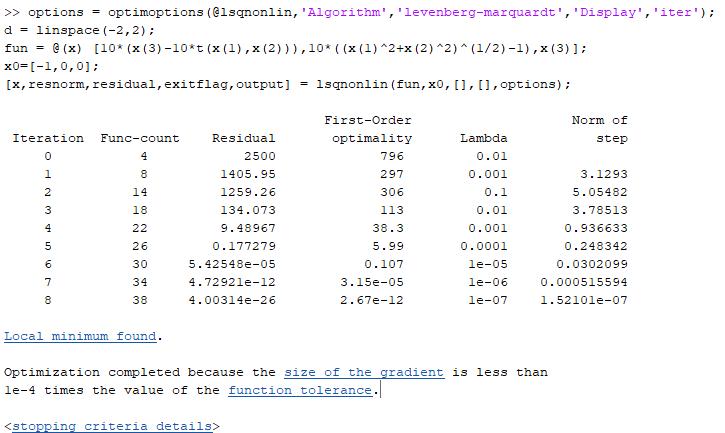
\includegraphics[width=0.9\textwidth]{imgs/lsqiter.png}
	\caption{Ejemplo de ejecución del comando \code{lsqnonlin} mostrando información sobre las iteraciones.}
	\label{fig:lsqnonlin-iter}
\end{figure}

Como vemos en la figura, se muestra información para cada iteración, donde \code{Func-count} es el número de evaluaciones de la función, \code{Resiudal} es el valor de la función objetivo, \code{First-Order optimality} es una medida de optimalidad de primer orden, \code{lambda} hace referencia a los multiplicadores de Lagrange y \code{Norm of step} es la norma del paso. Además, en la salida se guardan \code{[x,resnorm,residual,exitflag,output]}, que en orden son el punto final, la norma del valor de la función objetivo en el punto final, el valor de la función objetivo en el punto final, el código de salida y la información de salida, para más información ver \cite{lsqnonlin}.

Con el objetivo de entender mejor el funcionamiento del algoritmo y ponerlo en práctica, se ha implementado una versión simplificada de la descrita en el capítulo anterior con el propósito de compararla con el comando \code{lsqnonlin}. De aquí en adelante, cuando mostremos el comando \code{myLevMar} nos referimos a esta función, proporcionada en el Anexo \ref{chap:impl-simpl} que toma como argumentos \code{fun} y \code{x0}.

Para comenzar, veamos el ejemplo ya propuesto. El interés de este es la discontinuidad en el plano $x_1=0$, el cual se tiene que cruzar ya que definimos $x_0=(-1,0,0)$. En $x=(1,0,0)$ la suma de residuos vale $0$.

\begin{lstlisting}[style=Matlab-editor]
fun = @(x) [10*(x(3)-10*theta(x(1),x(2))),10*((x(1)^2+x(2)^2)^(1/2)-1),x(3)];
myX = myLevMar(fun,x0);
x = lsqnonlin(fun,x0,[],[],options);
\end{lstlisting}
La función \code{theta()} es la definida según (\ref{eq:theta}):
\vspace{10pt}
\begin{lstlisting}[frame=single, numbers=left, style=Matlab-editor]
function y = theta(x1,x2)
if x1 > 0
	y = 1/(2*pi)*atan(x2/x1);
else
	y = 1/(2*pi)*atan(x2/x1) + 0.5;
end
\end{lstlisting}

El resultado de la ejecución es el mismo para ambos, $x=(1,0,0)$. Para comprobar que la
implementación es correcta, la probamos ahora con otros ejemplos. El siguiente código es un ejemplo de la documentación de \code{lsqnonlin}
\cite{lsqnonlin} en el que se genera una muestra con un error aleatorio normalmente distribuído de media $0$. Este ejemplo es interesante porque la matriz jacobiana no es cuadrada como en el primer caso y nos sirve para ver que la implementación es funciona correctamente. El resultado se muestra en la figura \ref{out:exp}, también se muestran las curvas de $e^{-xt}$ con $x=2,3,4$ para ver mejor el efecto del ajuste.
\vspace{10pt}
\begin{lstlisting}[frame=single, numbers=left, style=Matlab-editor]
rng default % para que sea reproducible
d = linspace(0,3);
y = exp(-1.3*d) + 0.05*randn(size(d));
fun = @(r)exp(-d*r)-y;
x0 = 4;
x = myLevMar(fun,x0);
plot(d,y,'ko',d,exp(-x*d),'b-',d,exp(-4*d),'r:',d,exp(-3*d),'r:',d,exp(-2*d),'r:')
legend('Datos','Mejor ajuste','exp(-x*d) con x=2,3,4')
xlabel('t')
ylabel('exp(-tx)')
\end{lstlisting}

\begin{figure}[!ht]
	\centering
	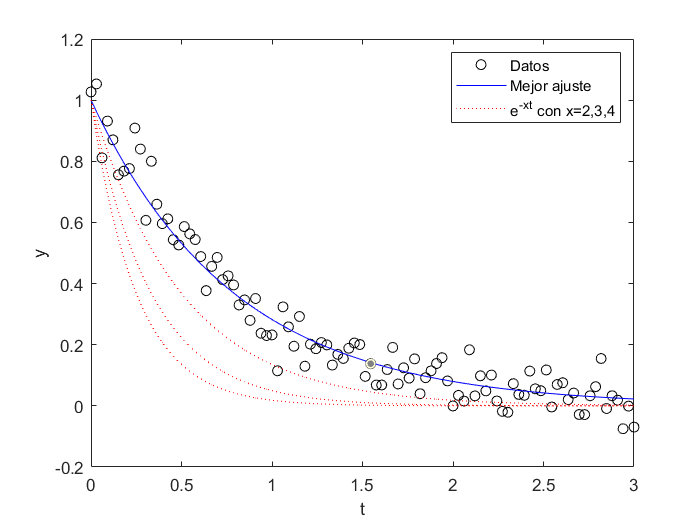
\includegraphics[width=0.7\textwidth]{imgs/exp.png}
	\caption{Resultado del ejemplo de ajuste exponencial.}
	\label{out:exp}
\end{figure}

Este es un ejemplo de estimación de parámetros en un modelo de regresión.
Se parte de unos datos muestrales y una función paramétrica que se cree que puede encajar con los datos, normalmente esta función se puede obtener por el contexto o, en su defecto, con alguna técnica de inferencia. En este caso se trata de la función $f(x)=e^{-xt}$, siendo $x$ el parámetro que queremos estimar. Para ello, definimos la función residuo $r(x)=e^{-xt}-y$, siendo $y$ los datos muestrales.



%%%%%%%%     Póñense a bibliografía, Apéndices e o índice alfabético     %%%%%%%%
\appendix
\renewcommand{\thechapter}{\Roman{chapter}}
\chapter{Código de la versión simplificada}\label{chap:impl-simpl}
Se muestra el código de Matlab\textsuperscript{®} para la implementación del algoritmo de Moré simplificado. Se presenta en forma de función \code{myLevMar} que toma como argumentos \code{fun} en forma de \textit{function handle} y \code{x0} el punto de partida. Se muestran las distintas funciones creadas para un código más limpio una tras otra. Para mayor comodidad, los archivos \code{.m} se pueden descargar desde el repositorio de Github \url{https://github.com/didacwhite/levenberg-marquardt} en la carpeta implementación.

\lstinputlisting[frame=single, numbers=left, style=Matlab-editor]{implementacion/myLevMar.m}
\lstinputlisting[frame=single, numbers=left, style=Matlab-editor]{implementacion/myLevMarSetup.m}
\lstinputlisting[frame=single, numbers=left, style=Matlab-editor]{implementacion/JDk.m}
\lstinputlisting[frame=single, numbers=left, style=Matlab-editor]{implementacion/jacob.m}
\lstinputlisting[frame=single, numbers=left, style=Matlab-editor]{implementacion/Jmfun.m}
\lstinputlisting[frame=single, numbers=left, style=Matlab-editor]{implementacion/pkfun.m}
\lstinputlisting[frame=single, numbers=left, style=Matlab-editor]{implementacion/hebden.m}
\lstinputlisting[frame=single, numbers=left, style=Matlab-editor]{implementacion/pk2.m}
\lstinputlisting[frame=single, numbers=left, style=Matlab-editor]{implementacion/rhofun.m}



\backmatter

%\begin{thebibliography}{99}

%%%%%%%%----Exemplo de entradas bibliográficas:
%

\bibliographystyle{amsplain}
%\nocite{*}
\bibliography{tfg, other}

%\end{thebibliography}




\end{document}


